
\chapter{Boundary conditions and well-posedness}\label{chap5}

\section{Introduction}\label{chap5:sec5.1}

We\pageoriginale have considered, so far, only initial value
probelms. We now turn to the situation when we have to solve a system
of equations in a domain which is bounded w.r.t. $x$, say $0 < x <
1$, and are given a certain initial-value function. In this case, we
look for appropriate boundary conditions on $x=0$ and $x =1$ which
will lead to the well-posedness of the problem. More precisely, we
look for boundary conditions which enable us to get energy estimates.

We illustrate the relevant ideas in the case of the three special
equations of section \ref{chap1}.

\section{The heat equation}\label{chap5:sec5.2}
 
Consider the simplest case of the  heat equation given by 
\begin{equation*}
\frac{\partial u}{\partial t} - \frac{\partial^2u}{\partial x^2} = 0,
\quad 0 < x < 1 \tag{5.1}\label{eq5.1}
\end{equation*}
with the initial condition $u(x,0) = u_\circ(x)$ being given.

We need boundary conditions on the lines $x =0$ and $x=1$. If
$\bar{n}$ is the outer normal on the boundary, we shall try to
maintain the same boundary conditions which work for the stationary
elliptic equation $\dfrac{\partial^2 u}{\partial x^2} =0$, i.e. we
write
\begin{equation*}
u + k \frac{\partial u}{\partial n} =0, \; k \geq 0, \tag{5.2}\label{eq5.2}
\end{equation*}
in case we look for a homogeneours boundary condition. Note that on
$x=1$, $\dfrac{\partial}{\partial n} = \dfrac{\partial}{\partial x}$ and
on $x=0$, $\dfrac{\partial}{\partial n} = \dfrac{-\partial}{\partial
  x}$. Thus (\ref{eq5.2}) can also be written as
\begin{equation*}
\left.
\begin{aligned}
u(1,t) + k_1 \frac{\partial u}{\partial x } (1,t) = 0, \; k_1 \geq 0\\
u(0 ,t) - k_\circ \frac{\partial u}{\partial x} (0,t) =0, \;
k_\circ \geq 0. \end{aligned} \right\}
\tag{5.3}\label{eq5.3}
\end{equation*}

We\pageoriginale now obtain an energy inequality. Multiplying (\ref{eq5.1}) by
$u$ and integrating w.r.t. $x$ from 0 to 1, one has 
$$
\int^1_0 u \frac{\partial u}{\partial t} dx - \int^1_0 u
\frac{\partial^2 u}{\partial x^2} dx = 0
$$
or, 
$$
\frac{1}{2} \frac{d}{dt} \int\limits^1_0 u^2 dx - u (1,t)
\frac{\partial u}{\partial x} (1,t) + u(0,1) \frac{\partial
  u}{\partial x} (0,t) + \int\limits^1_0 (\frac{\partial u}{\partial
  x})^2 dx = 0.
$$
Incorporating the conditions (\ref{eq5.3}), we get 
$$
\frac{1}{2} \frac{d}{dt} \int\limits^1_0 u^2 dx + \int\limits^1_0
\left(\frac{\partial u}{\partial x}\right)^2 dx + \frac{1}{k_1} u(1,t)^2 +
\frac{1}{k_\circ} u(0,t)^2 = 0,
$$
and, since the last three terms are non-negative, one gets,
$$
\frac{d}{dt} \int\limits^1_0 u^2 dx \leq 0,
$$
which leads to the energy estimate
\begin{equation*}
||u(\cdot, t) ||_2 \leq ||u(\cdot, 0)||_2 
\tag{5.4}\label{eq5.4}
\end{equation*}
where $||\cdot||_2$ denotes the norm in $L^2 (0,1)$. 

\section{The advection equation}\label{chap5:sec5.3}

We study the linear case where $u$ is a constant. The equation is
\begin{equation*}
\frac{\partial \varphi}{\partial t} + u \frac{\partial
  \varphi}{\partial x} = 0, \quad 0 < x <1
\tag{5.5}\label{eq5.5}
\end{equation*}
with given initial condition $\varphi (x,0) = \varphi_\circ (x)$.

We now ask ourselves if we can impose boundary conditions on $x=0$ and
$x=1$ freely. The answer comes from a consideration of the
characteristics.

Let us first consider the case where $u>0$. Then the characteristics
have positive slope. (Cf. Fig. \ref{c5:fig5.1}).

\begin{figure}[H]
\centering
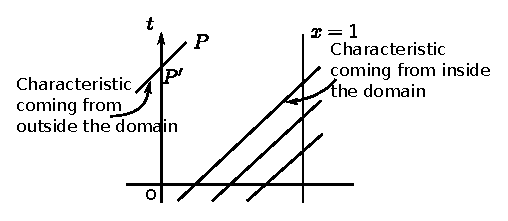
\includegraphics{figures/fig52-5.1.eps}
\caption{$(u > 0)$}\label{c5:fig5.1}
\end{figure}\pageoriginale

Since we know that $\varphi (x,t) = \varphi_\circ (x-ut)$, if we take
any point on $x=1$, with $0< t < \frac{1}{u}$, then the value of
$\varphi$ at this point is already determined, by the corresponding
value on $t=0$, on the same characteristic and we have no freedom of
imposing boundary conditions on $x=1$. 

On the other hand, if we impose a boundary condition  on $x=0$, then
for a point $P$ as in Fig. \ref{c5:fig5.1}, we can determine $\varphi(P) = \varphi
(P')$. Thus $\varphi$ will be completely determined in the domain
starting with the initial value $\varphi_\circ$ and the boundary
condition on $x=0$. 

If $u<0$, the roles of $x =0$ and $x=1$ are reversed. 

More generally, for a point on the boundary, if the characteristic
through that point comes from inside the domain, we cannot impose any
condition there. If it comes from outside (i.e. cuts $t=0$ outside the
domain) we can impose a suitable condition there. 

By our above arguments we showed that a boundary condition on $x=0$
determined $\varphi$ uniquely when $u>0$. We now show how to obtain an
energy estimate as well. Let us set the boundary condition
\begin{equation*}
\varphi(0,t) = g(t) \tag{5.6}\label{eq5.6}
\end{equation*}\pageoriginale
on the line $x=0$.

Multiplying (\ref{eq5.5}) by $\varphi$ and integrating w.r.t. $x$ over
$[0,1]$, we get 
$$
\frac{1}{2} \frac{d}{dt} \int\limits^1_0 \varphi^2 dx + \frac{u}{2}
(\varphi^2 (1,t) - \varphi^2 (0,t)) =0. 
$$
Integrating this w.r.t. $t$, we get
$$
\int\limits^1_0 \varphi^2 (x,t) dx - \int\limits^1_0 \varphi^2 
(x,0) dx + u \int\limits^t_0 \varphi^2  (1,s) ds - u
\int\limits^t_0 \varphi^2 (0, s) ds =0.
$$
Thus
$$
\int\limits^1_0 \varphi^2 (x,t) dx + u \int\limits^t_0 \varphi^2 (1,s)
ds = \int\limits^1_0\varphi^2 (x,0) dx + u \int\limits^t_0
\varphi^2 (0, s) ds 
$$
where the right-hand side is known and so is bounded. The second term
on the left is non-negative and one can omit it to get an energy
inequality for $||\varphi (\cdot, t)||_2$ in terms of known
quantities. 

\section{The wave equation-method of characteristics}\label{chap5:sec5.4}
We write down the wave equation as a system of two first order
equations:
\begin{equation*}
\begin{cases}
\dfrac{\partial u}{\partial t} + \dfrac{\partial v}{\partial x} = 0\\[5pt]
\dfrac{\partial v}{\partial t} + \dfrac{\partial u}{\partial x} = 0
\end{cases} \text{ in} \quad 0< x < 1 \tag{5.7}\label{eq5.7}
\end{equation*}
with the initial conditions, $u(x,0) = u_\circ(x)$, and $v(x,0) =
v_\circ (x)$. Adding these two equations we get
\begin{equation*}
\frac{\partial}{\partial t} (u+v) + \frac{\partial}{\partial x} (u+v)
= 0, \tag{5.8}\label{eq5.8}
\end{equation*}
and subtracting, one has
\begin{equation*}
\frac{\partial}{\partial t} (u-v) - \frac{\partial}{\partial x} (u-v)
= 0.  \tag{5.9}\label{eq5.9}
\end{equation*}

Thus,\pageoriginale through each point we have two characteristics
along which $u+v$ and $u-v$ are respectively constants,
(Cf. Fig. \ref{c5:fig5.2}).

\begin{figure}[H]
\centering
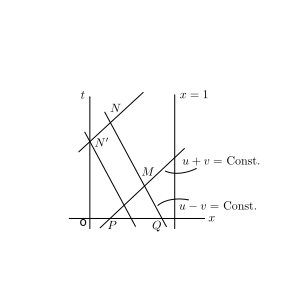
\includegraphics{figures/fig52-5.2.eps}
\caption{}\label{c5:fig5.2}
\end{figure}

For a point $M$ as in the above figure, both $u+v$ and $u-v$ are known
from the corresponding values at $P$ and $Q$, and hence $u, \; v$ can
also be uniquely computed at $M$. On the other hand consider the
points $N$ and $N$'. For these one only knows $u-v$ from the initial
conditions. If we impose a boundary condition on $x=0$ so that we can
solve for $u+v$ and $u-v$, then $u$ and $v$ can also be uniquely
computed.

To this end we impose a boundary condition of the type
\begin{equation*}
u(0,t) + \alpha v(0,t) = 0, \quad \alpha \neq -1 \tag{5.10}\label{eq5.10}
\end{equation*}
on $x=0$. Then knowing $u-v$ at $N'$, together with (\ref{eq5.10}) we can
compute $u$ and $v$ at $N'$. Hence we know $u+v$ and $u-v$ at $N'$ and
at $N$, from which we calculate $u$ and $v$ at $N$, uniquely.

Similar arguments show that the boundary condition on $x=1$ could be 
\begin{equation*}
u(1,t) + \beta v(1,t ) = 0, \beta \neq 1. \tag{5.11}\label{eq5.11}
\end{equation*}

Thus the conditions (\ref{eq5.10}) and (\ref{eq5.11}) help us to
compute the solution  uniquely\pageoriginale in the entire domain.  

More generally, to get the boundary conditions by the {\em method of
  characteristics}, we take any point on the boundary and draw the $n$
characteristics (for a hyperbolic system of $n$ equations) through the
point. If $p$ of them come from outside, we may impose $p$ boundary
conditions in such a way as to be independent of each other, as well
as the $n-p$ relations already given by the characteristics from
inside so that, we can solve for the solution in the entire domain.

However it must be noted that by this method we do not get any energy
estimate which is a key step in the study of well-posedness.

\section{The wave equation-Friedrichs' method}\label{chap5:sec5.5}

In order to get an energy estimate to study the well-posedness, we
turn to Friedrichs' method for symmetric systems to find the
appropriate boundary conditions. We specialize to the simplest case,
and refer the interested reader to Friedrichs \cite{key10}.

Consider the system of $n$ equations
\begin{equation*}
\frac{\partial U}{\partial t} + A \frac{\partial U}{\partial x} = 0,
\quad 0< x < 1\tag{5.12}\label{eq5.12}
\end{equation*}
with the initial condition  $U(x,0) = U_\circ(x)$, and such that
the matrix $A(x,t)$ is symmetric.

Define a matrix $B(t)$ by 
\begin{equation*}
\left. 
\begin{aligned}
B_1 (t) & = A(1,t)\\
B_\circ (t) & = -A (0, t)
\end{aligned} \right\}
\tag{5.13}\label{eq5.13}
\end{equation*}
on the boundary. We introduce also a matrix $M(t)$ (which is $M_1(t)$
on $x=1$ and $M_\circ(t)$ on $x=0$) which has the following properties:
\begin{equation*}
\left.
\begin{aligned}
{\rm (i)}  \qquad & M + M^T \text{ is positive semi-definite},\\
{\rm (ii)} \qquad & \Ker (B+M) \oplus \Ker (B-M) = \mathbb{R}^n. 
\end{aligned}
\right\}
\tag{5.14}\label{eq5.14}
\end{equation*}\pageoriginale

Then the Friedrichs' boundary condition is that $U \in \Ker (B-M)$ on
the boundary. Assuming $A$ to be a constant matrix, we derive an
energy inequality. Taking the scalar product of (\ref{eq5.12}) with $U$ and
integrating w.r.t. $x$ over $[0,1]$, one has
\begin{equation*}
\int\limits^1_0 \left(\left\langle U, \frac{\partial U}{\partial
  t}\right\rangle + \left\langle U, \; A \frac{\partial U}{\partial x}
\right\rangle\right) dx =0. 
\tag{5.15}\label{eq5.15}
\end{equation*}
Using the symmetry of $A$ and the fact that $A$ is constant, (\ref{eq5.15})
can be written as
$$
\frac{1}{2} \frac{d}{dt} \int\limits^1_0 |U|^2 dx + \frac{1}{2}
\int\limits^1_0 \frac{\partial}{\partial x} \langle U, AU\rangle dx = 0.
$$
Or,
\begin{equation*}
\frac{d}{dt} \int\limits^1_0 |U|^2 dx + \langle U, AU \rangle_{x=1} -
\langle U, AU\rangle_{x=0} = 0. \tag{5.16}\label{eq5.16}
\end{equation*}
Using the relations (\ref{eq5.13}) and the fact that $U \in \ker (B-M)$, one
has 
\begin{align*}
\langle U, AU\rangle _{x=1} - \langle U, AU\rangle {}_{x=0} & =
\langle U, B_1 U \rangle  + \langle U, B_\circ U\rangle \\
\langle U, M_1 U \rangle  + \langle U, M_\circ U \rangle .
\end{align*}
But
\begin{align*}
\langle U, MU\rangle & =  \langle M^T U, U\rangle = \langle U, M^TU\rangle \\
& = \frac{1}{2} \langle U, MU \rangle + \frac{1}{2}\langle  U, M^TU\rangle \\
& = \frac{1}{2} \langle  U, (M+M^T) U\rangle \\
& \geq 0
\end{align*}
by virtue of (\ref{eq5.14}) (i).

Using this in (\ref{eq5.16}) (i), we get the condition 
$$
\frac{d}{dt} \int\limits^1_0 |U|^2 dx \leq 0
$$\pageoriginale
or, following the notation of Sec. \ref{chap4:sec4.1},
\begin{equation*}
|| U(\cdot, t)||^2 \leq ||U(\cdot, 0)||^2, 
\tag{5.17}\label{eq5.17}
\end{equation*}
which is an energy inequality.

\begin{remark}\label{chap5:rem5.1}
We have not used the condition (\ref{eq5.14}) (ii) at all. This is used in
proving the existence of solution, for which one has to work with the
adjoint problem.
\end{remark}

\section{Comparison of the preceding methods}\label{chap5:sec5.6}

Observe that the case of the wave equation (\ref{eq5.7}) falls within the
framework of Friedricns' theory if we take 
$$
A = \begin{bmatrix} 
0 & 1\\ 
1 & 0
\end{bmatrix}.
$$

\begin{exercise}\label{chap5:exer5.1}
Find all matrices $M$ which satisfy the conditions (\ref{eq5.14}) w.r.t. the
above matrix $A$ and compare the Friedrichs' boundary condition with
the boundary conditions (\ref{eq5.10}) and (\ref{eq5.11}).
\end{exercise}

The solution of exercise \ref{chap5:exer5.1} will reveal that the Friedrichs'
conditions are more restrictive. The advantage of Friedrichs' method
lies in the fact that we get an energy estimate in this case while we
could not get one by the method of characteristics. 

Another interesting question is whether Friedrich's boundary
conditions, though restrictive, ar equal in number to those got by
the method of characteristics.

We show that this is the case in a very particular situation. (The
general\pageoriginale case is still open, to the best of the knowledge
of the author).

Assume that $B$ is symmetric and regular. Diagonalizing it by an
orthogonal matrix $Q$, one has 
$$
B_1 = Q D Q^T.
$$
Choose $M = Q |D| Q^T$. Thus,
\begin{align*}
B_1 + M & = Q (D + |D|) Q^T\\
B_1 - M & = Q (D - |D|) Q^T.
\end{align*}
If $D = \text{ diag } \left\{ \lambda_1, \ldots \lambda_k, \; -
\lambda_{k+1} , \ldots, -\lambda_n\right\}$ where $\lambda_i > 0$ for
all $i$, then
\begin{align*}
\Ker (B_1 -M) & = Q \Ker (D-|D|) Q^T\\
& = \left\{ U|V = Q^T U \text{ with } V_{k+1} = \ldots = V_n = 0 \right\}.
\end{align*}
Similarly,
\begin{align*}
\Ker (B_1+M) & = Q \Ker (D+|D|)Q^T\\
& = \left\{ U|V = Q^T U, \text{ with } V_{k+1} = \ldots = V_n =
0\right\}. 
\end{align*}

On the boundary $x=1$, $B (=+A)$ has $k$ eigenvalues $ >0$. Thus $n-k$
characteristics come from outside and we should have $n-k$
conditions. One the other hand $U \in \Ker (B-M) = Ker (D-|D|)$ also
gives $n-k$ conditions.

Similarly one can argue for $B_\circ = - B_1$ on $x=0$.

A final word on the wave equation. One can also write the equation as
one of second order in the form
\begin{equation*}
\frac{\partial^2 w}{\partial t^2} - \frac{\partial^2 w}{\partial x^2}
= 0, \quad 0 < x < 1. \tag{5.18}\label{eq5.18}
\end{equation*}

By the substitutions
\begin{equation*}
u = \frac{\partial w}{\partial t}; \; v  = - \frac{\partial
  w}{\partial x}, \tag{5.19}\label{eq5.19}
\end{equation*}\pageoriginale
we can retrieve the system (\ref{eq5.7}).

One of the types of boundary conditions one can impose on (\ref{eq5.18}) is
the same as for the stationary elliptic problems, i.e.
\begin{equation*}
w + k \frac{\partial w}{\partial n} = 0, \; k \geq 0,
\tag{5.20}\label{eq5.20}
\end{equation*}
where $\bar{n}$ is the outer normal on the boundary.

\begin{exercise}\label{chap5:exer5.2}
Find an energy estimate for the solution of (\ref{eq5.18}) with the boundary
condition  (\ref{eq5.20}).
\end{exercise}

However there is one other boundary condition which we state in 

\begin{exercise}\label{chap5:exer5.3}
Using the boundary condition
\begin{equation*}
\frac{\partial w}{\partial t} + k \frac{\partial w}{\partial n} = 0,
\; k \geq 0,\tag{5.21}\label{eq5.21}
\end{equation*}
find an energy estimate for the solution of (\ref{eq5.18}). Using the
substitutions (\ref{eq5.19}) compare this boundary condition with that of
Friedrichs or that got by the method of characteristics for the system
(\ref{eq5.7}). 
\end{exercise}

All this work has been done only when the equations are linear and
involve one space variable. Kreiss has done some work in the
2-dimensional case.

For non-linear problems, one linearizes the problem around the
bou\-ndary to find out appropriate boundary conditions. As usual, the
number of characteristics from outside give as many boundary
conditions which must be chosen independent of themselves as well as
of the relations given by those characteristics from inside.

